\paragraph{Алгоритм оценки АКФ}
Точность АР метода напрямую зависит от точности оценки АКФ гармонического сигнала.
Существует несколько способов компенсации шума для АР анализа \cite{kay_ar_book}.
Основным способом повышения точности оценки АКФ является увеличение размера выборки, что в случае модулированного сигнала может быть затруднительным. 

В данной работе предлагается использовать алгоритм увеличения отношения сигнал-шум методом последовательного вычисления АКФ \cite{ostanin_akf}.
Для снижения вычислительных затрат последовательное вычисление АКФ предлагается реализовывать с использованием процедуры БПФ. 
Введем следующие обозначения: ${x}$ – вектор входного сигнала после снятия ПСП, ${F}$ – матрица прямого преобразования Фурье,
${F^{-1}}$ - матрица обратного преобразования Фурье. Оценку АКФ на первом шаге можно получить следующим образом:

\begin{equation}
	\label{eq:akf_akf}
	\hat{r}_1 = F^{-1}\left[ Fx \cdot (Fx)^* \right] = F^{-1} \left[ \left| Fx \right| ^2 \right]
\end{equation}
Здесь знак ${(\cdot)}$  означает поэлементное перемножение векторов, ${\left| Fx \right| ^2}$ - поэлементное возведение модуля комплексного числа в квадрат, ${*}$ - означает
комплексное сопряжение.  Следуя алгоритму, изложенному в \cite{ostanin_akf} вычислим оценку АКФ от ${\hat{r}_1}$:

\begin{center}
\begin{eqnarray}
	\label{eq:akf_2}
	\hat{r}_2 & = & F^{-1}\left[ F \hat{r}_1 \cdot (F \hat{r}_1)^* \right] = \nonumber \\
		& = & F^{-1}	\left[ 
				FF^{-1} \left[
						\left| Fx \right| ^2
					\right]
						\cdot \left( FF^{-1} \left[ \left| Fx \right| ^2 \right]
					\right) ^*
			\right] = \nonumber \\
		& = & F^{-1} \left[ \left| Fx \right| ^2 \cdot \left[ \left| Fx \right| ^2 \right] ^* \right] =  \nonumber \\
		& = & F^{-1} \left[ \left| Fx \right| ^4 \right]
\end{eqnarray}
\end{center}

Рассуждая аналогично, можно показать, что уточненная оценка АКФ на K-ом шаге алгоритма, рассмотренного в \cite{ostanin_akf}
может быть получена без использования итераций с помощью выражения:
\begin{center}
\begin{equation}
	\label{eq:akf_3}
	\hat{r}_K = F^{-1}\left[ \left| Fx \right| ^{2^K} \right]
\end{equation}
\end{center}

Схематически алгоритм получения уточненной оценки АКФ на третьем шаге представлен на рисунке \ref{pic:akf_pic}.
\begin{figure}[H]
	\center\scalebox{0.8}{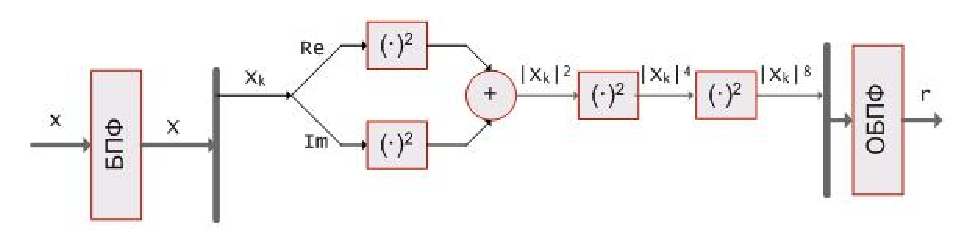
\includegraphics[width=1\linewidth]{akf_fft.eps}}
	\caption{Усовершенствованный итеративный алгоритм получения АКФ}
	\label{pic:akf_pic}
\end{figure}

Количество умножений необходимых для оценки АКФ прямым методом: ${OP_{ACF} = 3N^2}$. Количество умножений необходимых для оценки
усовершенствованным итеративным алгоритмом получения АКФ: ${OP_{ACF\_FFT} = 8NlogN + (k+2)N}$.

Увеличение отношения ОСШ в оценке АКФ по мощности можно вычислить по формуле представленной в \cite{book_max}:
\begin{center}
\begin{equation}
	\label{eq:akf_max_eq}
	G=2BT \frac{1}{2+1/SNR_k}
\end{equation}
\end{center}
где ${G=\frac{SNR_{k+1}}{SNR_k}}$ - относительный прирост ОСШ, ${T}$ - длинна выборки (сек), ${B}$ -  ширина спектра сигнала, 
а ${SNR}$ - ОСШ.

Из \ref{eq:akf_max_eq} видно, что увеличение ОСШ при вычислении оценки АКФ пропорционально ${2BT}$ и зависит от
ОСШ на входе коррелометра, так же можно отметить, что увеличение ОСШ происходит только при условии ${BT > \frac{1}{2SNR_k} + 1}$.
